\graphicspath{%
{chapter2graph/}%
{chapter2graph/bg/}}
%\makeindex


\chapter{Metrics}

\section{Variance, $\sigma^2$ or Var($X$)}

Variance is the expectation of the \underline{squared} deviation of a random variable from its \underline{mean}.  Note that the unit of variance is the square of the variable's unit. \\

1) discrete random variable\\
This is for discrete random variable (applicable to most dataset), if the generator of random variable $X$ is discrete with Probability Mass Function (PMF) that maps value $x_i$ to probability $p_i$, (certain $x_i$ and $p_i$ pairs can be same value due to same $x$ value in the dataset) then the variance will be:
\begin{eqnarray}
Var(X) = \sum_{i=1}^{n} p_i (x_i - \mu)^2
\label{variancedis}
\end{eqnarray}
where $\mu$ is the expected value:
\begin{eqnarray}
\mu = \sum_{i=1}^{n} p_i x_i
\label{expected}
\end{eqnarray}

If the each value in the $n$ data points are equally likely, then the variance will be:
\begin{eqnarray}
Var(X)= \frac{1}{n}\sum^{n}_{i=1}(x_i - \mu)^2
\label{variancediseq}
\end{eqnarray}

2) continuous random variable\\
If the random variable $X$ has a Probability Density Function (PDF) $f(x)$, then the variance will be:
\begin{eqnarray}
Var(X) = \int_{\mathbb{R}} (x - \mu)^2 f(x) dx
\label{variancecon}
\end{eqnarray}
where $\mu$ is the expected value:
\begin{eqnarray}
\mu = \int_{\mathbb{R}} xf(x)dx
\label{expectedcon}
\end{eqnarray}

\section{Standard Deviation, $\sigma$}

The standard deviation is a measure of the amount of variation or dispersion of a set of values. For both discrete and continuous random variable, the standard deviations are $\sqrt{\text{variance}}$ and note that this quantity has the same physical units as the random variable. \\

\section{Standard Error}

The standard error is a type of standard deviation for the distribution of the means. \\

There will be, of course, different means for different samples (from the same population), this is called “sampling distribution of the mean”. This variance between the means of different samples can be estimated by the standard deviation of this sampling distribution and it is the standard error of the estimate of the mean. Standard error measures the precision of the estimate of the sample mean. The standard error is strictly dependent on the sample size and thus the standard error falls as the sample size increases. It makes total sense if you think about it, the bigger the sample, the closer the sample mean is to the population mean and thus the estimate of it is closer to the actual value.
\begin{eqnarray}
\text{Standard Error} = \frac{\sigma}{\sqrt{n}}
\label{se}
\end{eqnarray}
where $\sigma$ is the standard deviation of the population (although sometimes population standard deviation is unknown, we can replace it with sample standard deviation as an estimate) and $n$ is the size (number of observations) of the sample.

\section{Confusion Matrix}

The confusion matrix is a table specifically for the problem of statistical classification. A typical confusion matrix table is shown below:

\begin{figure}[h!]
\begin{center}
	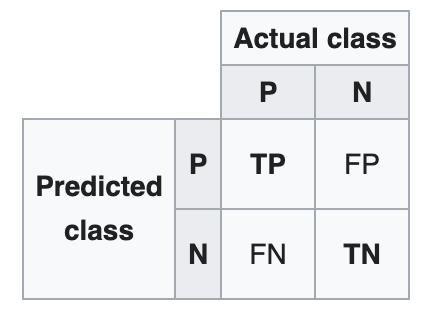
\includegraphics[scale=0.5]{confuse.png}
	\caption[]{Confusion Matrix}
	\label{confusing}
	\end{center}
	\end{figure}

where:\\
TP : True Positive or Hit \\
TN : True Negative or Correct Rejection\\
FP : False Positive or Type I error\\
FN : False Negative or Type II error\\

A more graphical way of seeing this is shown in Fig. (\ref{precisionrecall}).
\begin{figure}[h!]
\begin{center}
	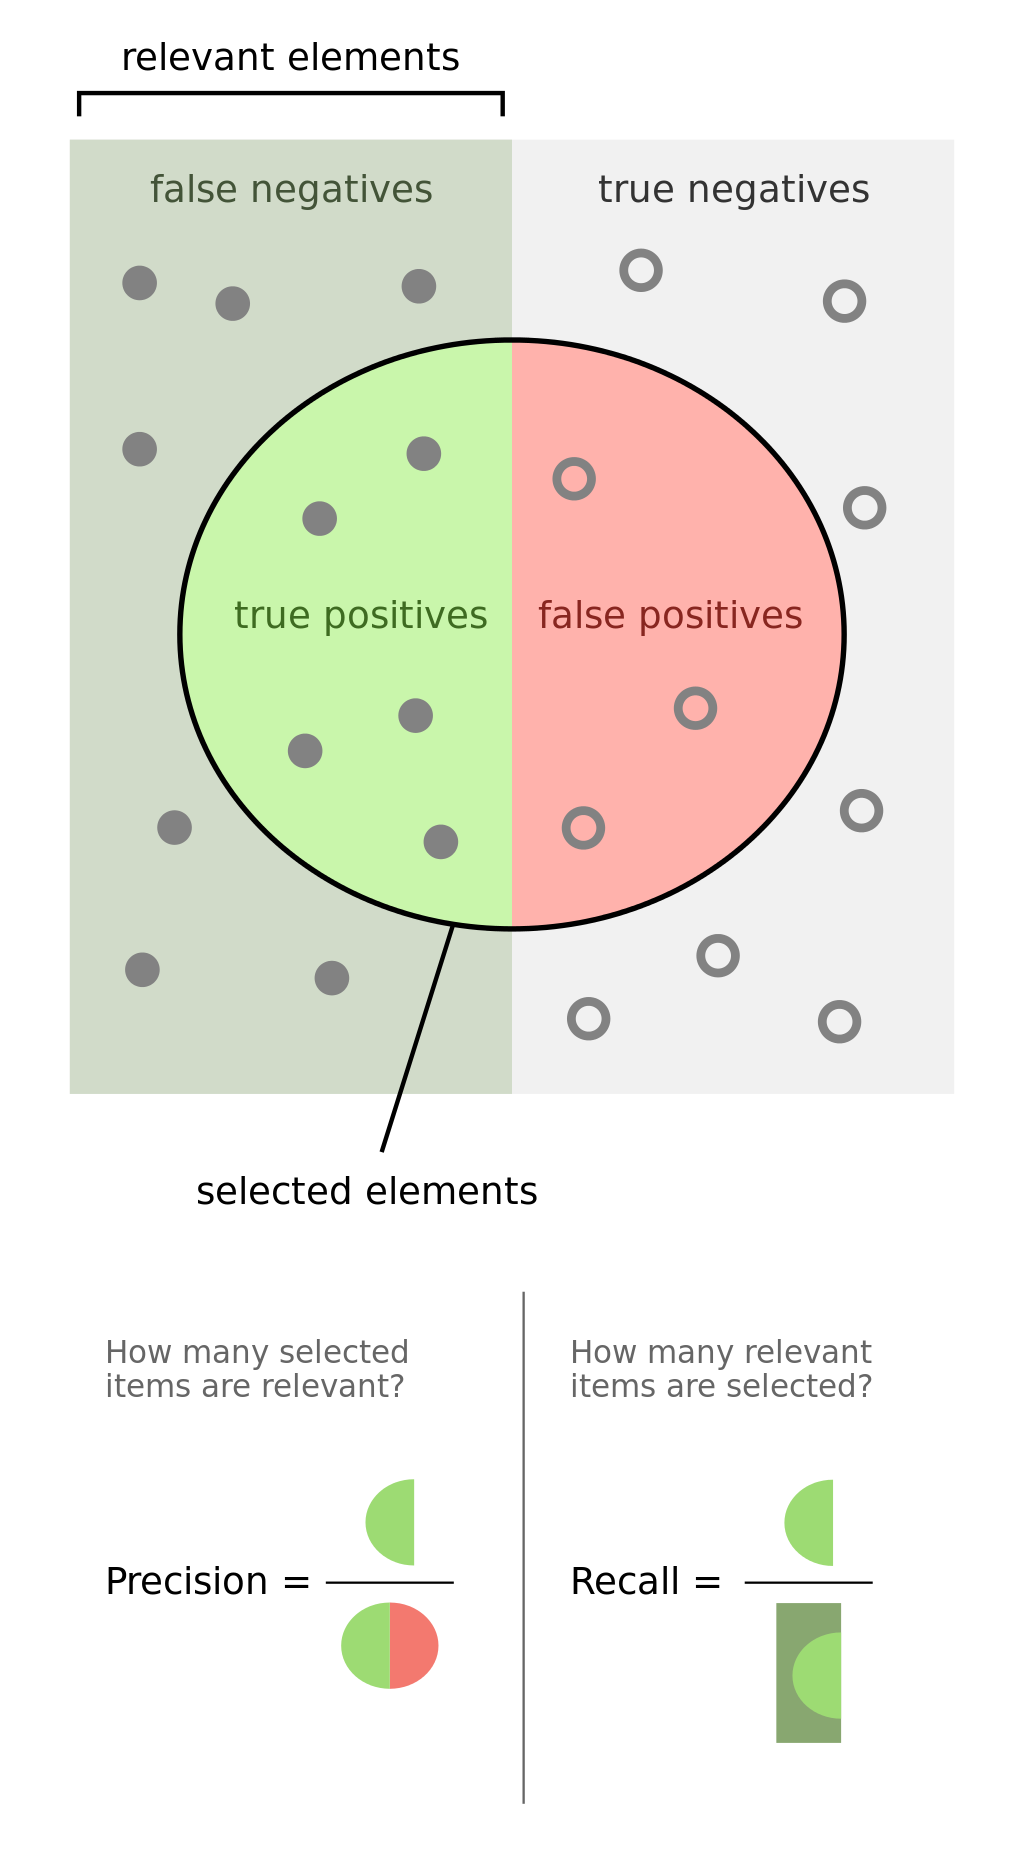
\includegraphics[scale=0.15]{precisionrecall.png}
	\caption[]{Graphical representation of confusion matrix}
	\label{precisionrecall}
	\end{center}
	\end{figure}
	
	
	
\subsection{Recall}

Recall is also called Sensitivity or True Positive Rate (TPR), it measures how many relevant items are selected (among the total numbers of relevant elements):
\begin{eqnarray}
\text{Recall} = \frac{\text{True Positive}}{\text{True Positive}+\text{False Negative}}
\label{recall}
\end{eqnarray} 

\subsection{Precision}

Precision is also called Positive Predictive Value (PPV), it measures how many selected items are relevant:
\begin{eqnarray}
\text{Precision} = \frac{\text{True Positive}}{\text{True Positive}+\text{False Positive}}
\label{precision}
\end{eqnarray} 

\subsection{$F_1$}

The $F_1$ score is a measure of a test's accuracy. It is basically the harmonic mean of the precision and recall. The highest possible $F_1$ score is 1, indicating perfect precision and recall, and the lowest possible score is 0, if either precision or recall is 0.
\begin{eqnarray}
F_1 = 2 \times \frac{\text{precision}\times\text{recall}}{\text{precision} + \text{recall}}
\label{f1}
\end{eqnarray} 

\section{ROC}

The Receiver Operating Characteristic Curve, or ROC curve, is a graphic plot that illustrates the diagnostic ability of a binary classifier system as its \underline{discrimination threshold is varied}. \\

To obtain the ROC curve, we need to plot the True Positive Rate (TPR) against the False Positive Rate (FPR):\\
True Positive Rate (TPR): also known as Sensitivity, Recall.\\
False Positive Rate (FPR): $\frac{\text{FP}}{\text{FP}+\text{TN} \text{(i.e. total actual negative)}}$, and is basically $1 - \text{Specificity}$.\\


In an ROC curve, the best possible prediction model would yield a point (for a certain discrimination threshold) in the upper left corner. This represent $100\%$ Recall (No False Negative) and $100\%$ Specificity (No False Positive). A \underline{random guess} would give a point along a diagonal line. An intuitive example of random guessing is a decision by flipping coins. As the size of the sample increases, a random classifier's ROC point tends towards the diagonal line, specifically for the case of a fair coin, it will tend to the point (0.5, 0.5)\\

The diagonal divides the ROC space. Points above the diagonal represent good classification results (better than random); points below the line represent bad results (worse than random). The table below shows 4 prediction model for 100 positive and 100 negative instances:

\begin{figure}[h!]
\begin{center}
	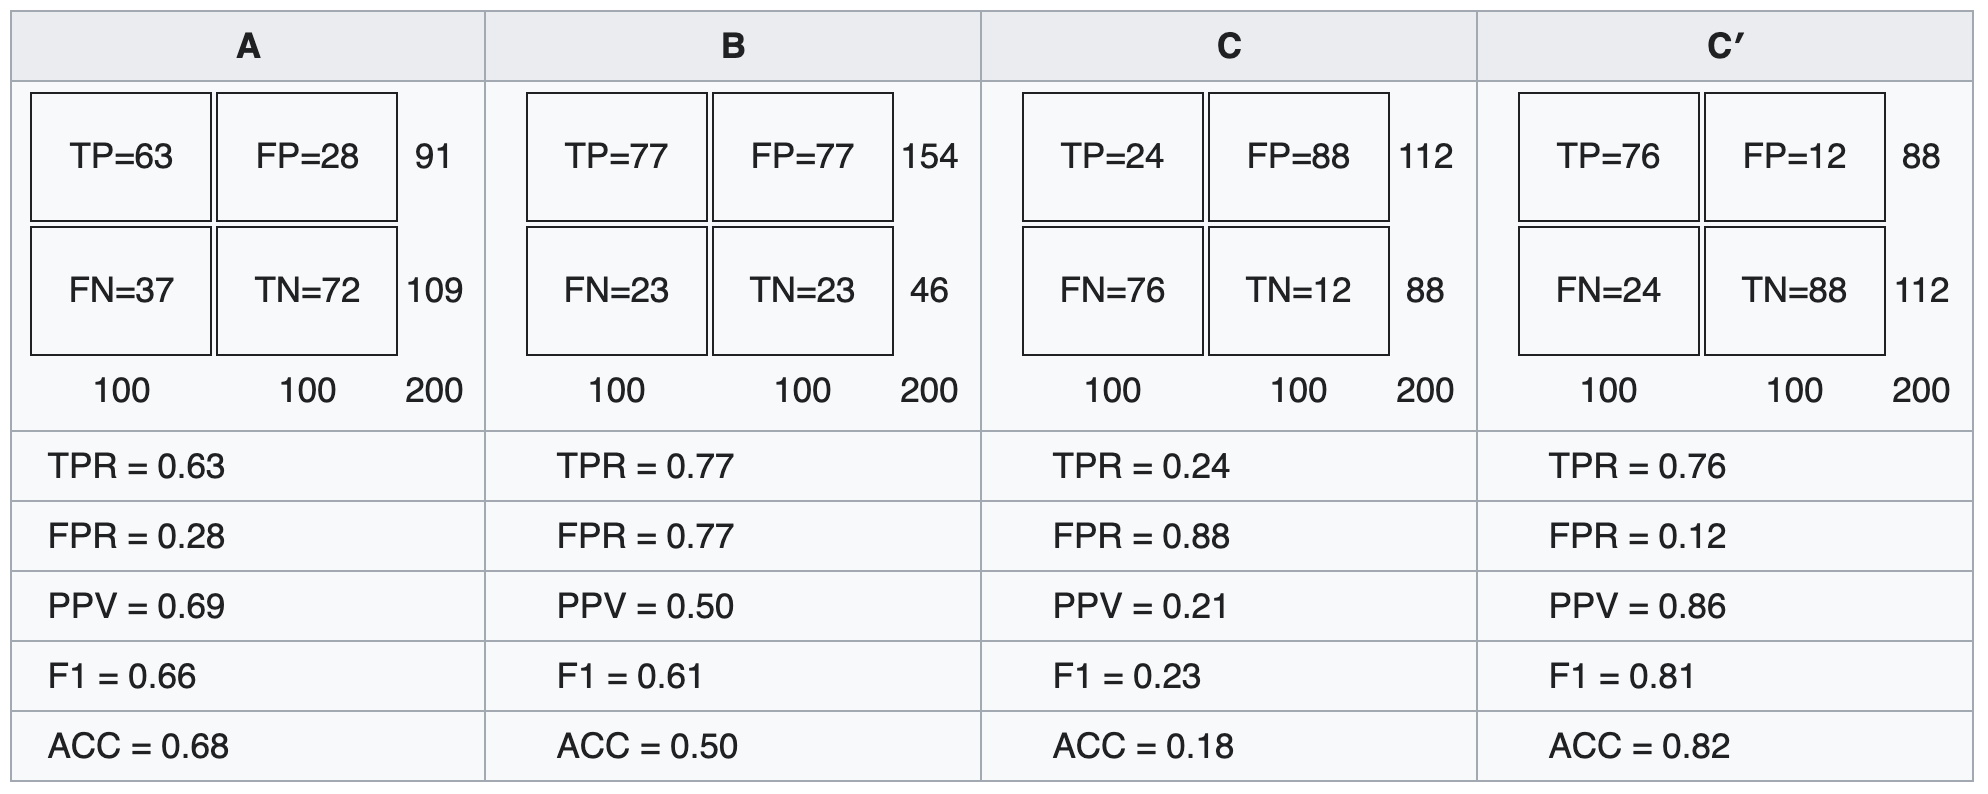
\includegraphics[scale=0.4]{roc_models.png}
	\caption[]{The prediction from 4 models, each at a certain discrimination threshold.}
	\label{precisionrecall}
	\end{center}
	\end{figure}
	
Plots of the four models in the ROC space is given below. The result of A clearly shows the best predictive power among A, B, C. The result from B lies on the random guess line, and it can be seen in the table that the accuracy of B is $50\%$. However, when C is mirrored across the center point (0.5, 0.5), the resulting model C' is even better than A. This mirrored method simply reverse the predictions from C. \\

\begin{figure}[h!]
\begin{center}
	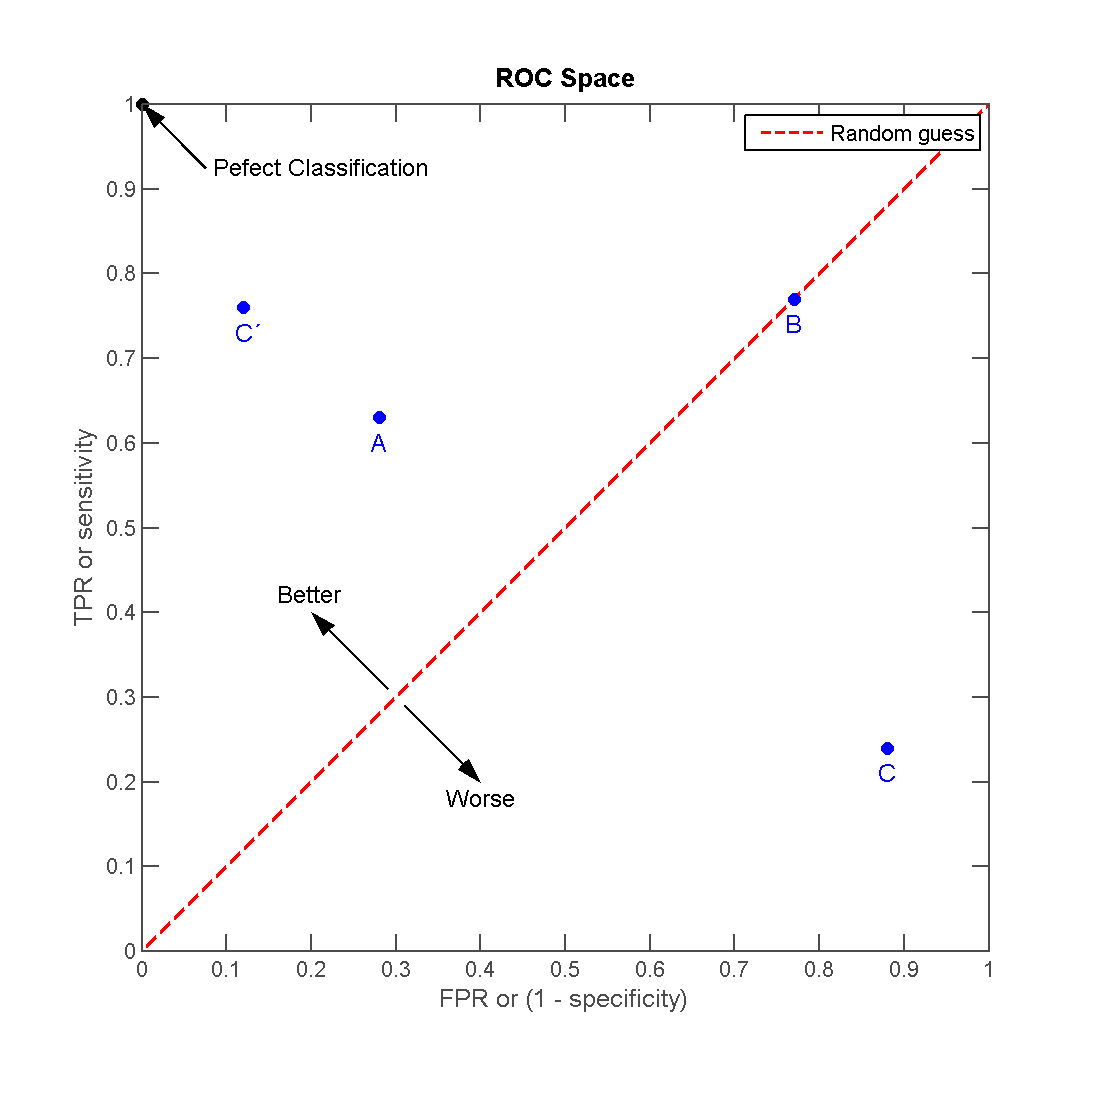
\includegraphics[scale=0.5]{ROC_space.png}
	\caption[]{The prediction from 4 models, each at a certain discrimination threshold.}
	\label{precisionrecall}
	\end{center}
	\end{figure}
	
The closer the model can be at towards the upper left corner, the better. But the distance from the random guess line in either direction is the best indicator of how much predictive power a method has. If the result is below the line, all of the model's predictions must be reversed in order to utilize its power. Note that the output of a consistently bad predictor could simply be inverted to obtain a good predictor.

\subsection{In the context of logistic regression}

For binary classification, given certain features, logistic regression will output a probability $p$, with respect to the target variable.\\
if $p$ > 0.5, we label the data as 1;\\
if $p$ < 0.5, we label the data as 0;\\
By default the threshold is 0.5.\\

When the threshold = 0 , the model will predict 1 for all, which means that both TPR and FPR will be 1.\\
When the threshold = 1, the model will predict 0 for all, which means that both TPR and FPR will be 0.\\

If we vary the threshold between these 2 extremes, we will have a series of TPR and FPR pairs. If we try all possible threshold then we can map out the ROC curve for this particular model.

 \begin{figure}[h!]
\begin{center}
	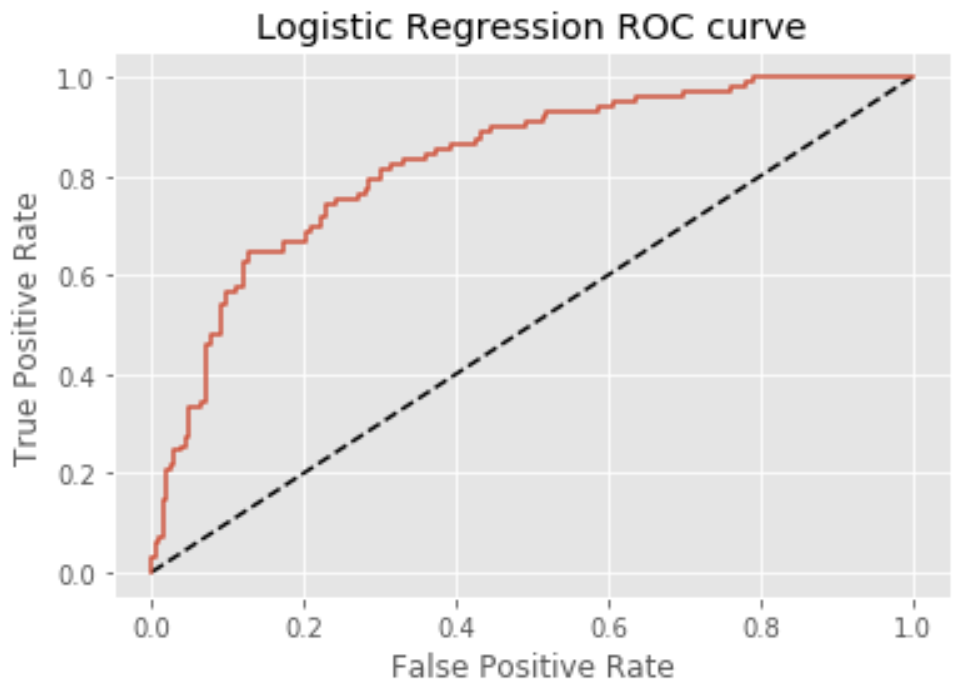
\includegraphics[scale=0.5]{lr_roc.png}
	\caption[]{ROC curve for a logistic regression model.}
	\label{precisionrecall}
	\end{center}
	\end{figure}
	
When using normalised unit, the area under the curve (AUC) is the probability that a classifier will rank a randomly chosen positive instance higher than a randomly chosen negative ones. (assuming that positive rank higher than negative in the dataset).
	
\section{Covariance}

The covariance is a measure of the joint variability of two random variables. If the greater values of one variable mainly correspond with the greater values of the other variable, and the same holds for the lesser values, (i.e. the variables tend to show similar behaviour), then the covariance is positive. In the opposite case, when the greater values of one variable mainly correspond to the lesser values of the other (i.e. the variables tend to show opposite behaviour), then the covariance is negative.

\begin{figure}[h!]
\begin{center}
	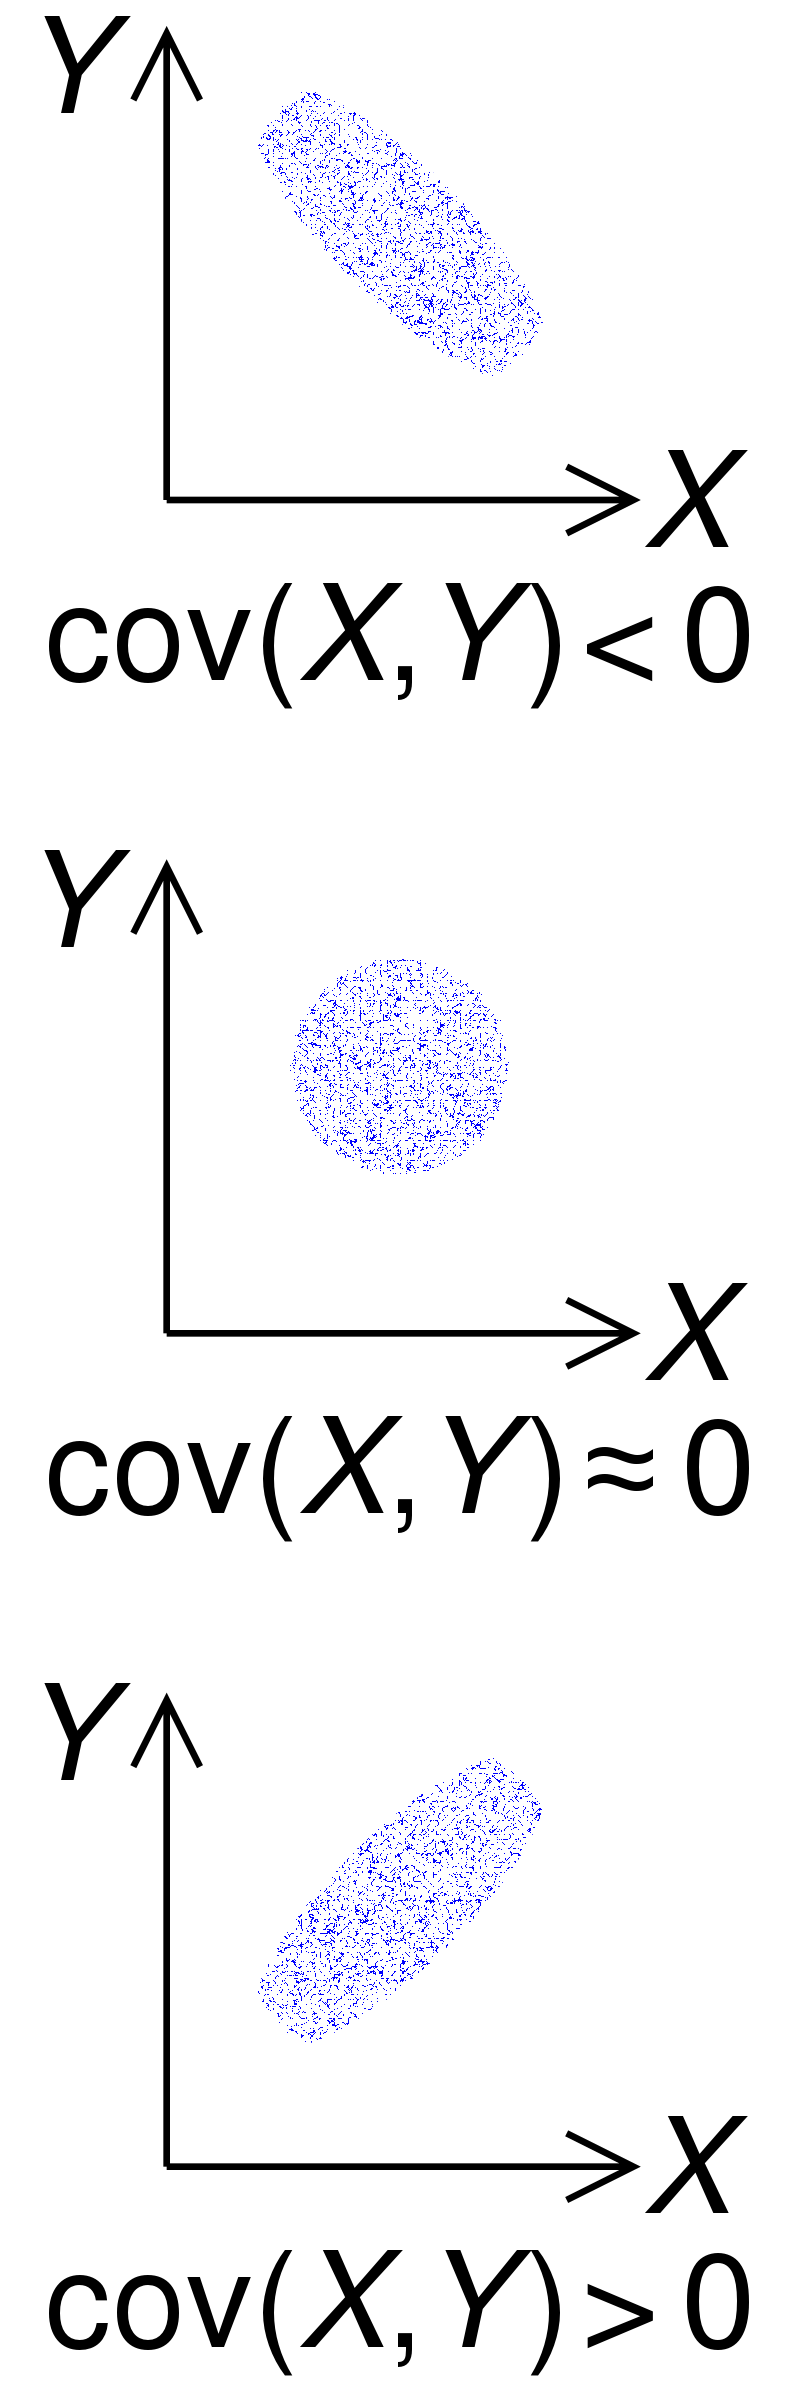
\includegraphics[scale=0.1]{covariance_trends.png}
	\caption[]{The sign of the covariance of two random variables $X$ and $Y$.}
	\label{precisionrecall}
	\end{center}
	\end{figure}
	
The description above is for covariance of two random variables. We also have sample covariance. The formula to calculate covariance is:\\
\begin{eqnarray}
\text{covariance} = \frac{1}{n} \sum^{n}_{i =1} (x_i - \mu_x)(y_i - \mu_y)
\label{covariance}
\end{eqnarray}
where $\mu_x$ and $\mu_y$ are the mean of $x$ and $y$ in the dataset. When both $x$ and $y$ increase or decrease together, then they are positively correlated.

\section{Pearson's Correlation Coefficient}

The correlation or dependence is any statistical relationship, whether causal or not, between two random variables or bivariate data. The most familiar measure of dependence between two quantity is the \underline{Pearson product-moment correlation coefficient}, or Pearson's Correlation Coefficient. This coefficient is dimensionless and takes value between (-1, 1). The correlation coefficient is +1 in the case of a perfect directly (increasing) linear relationship, -1 in the case of a perfect inverse linear relationship. \\

If the variables are independent, Pearson's Correlation Coefficient is 0. But the converse is not true, because the correlation coefficient detects only linear dependencies between two variables.\\

The Pearson Correlation Coefficient $\rho_{X,Y}$ between two random variables $X$ and $Y$ with standard deviation $\sigma_X$ and $\sigma_Y$ is defined as:
\begin{eqnarray}
\rho_{X,Y} = \frac{\text{covariance($X$, $Y$)}}{\sigma_X \sigma_Y}
\label{pearson}
\end{eqnarray}
The Pearson Correlation is only defined only if both standard deviation are finite and positive. 


\section{Confidence Interval}

\section{Confidence Level}

\section{P value}

See Chapter (\ref{abtest})

\section{T value/t-statistic}

The t-statistics 
See Chapter (\ref{ttest})

\section{Z value}

Details please see Chapter (\ref{ztest}).\\

Z value, also known as z-scores and more commonly the Standard Score, is the number of standard deviations by which the value of a raw score (i.e. an observed value or data point) is above or below the \underline{mean} value of what is being observed or measured. Raw scores above the mean have positive z value, while those below the mean have negative z value. \\

If the population mean and population standard deviation are known, a raw score $x$ is converted to z score by:
\begin{eqnarray}
z = \frac{x - \mu}{\sigma}
\label{zscore}
\end{eqnarray}
where:\\
$\mu$ is the mean of the population and $\sigma$ is the standard deviation of the population. Calculating z score using this formula requires the population mean and population standard deviation, NOT the sample mean or sample deviation.  But knowing the true mean and standard deviation of a population is often unrealistic except in cases such as standardised testing, where the entire population is measured. \\

When the the population standard deviation are unknown, the z score may be calculated using sample standard deviations as estimates of the population. In these case, sometimes the z score is normalised by the sample size:
\begin{eqnarray}
z = \frac{x - \bar{x}}{\bar{\sigma}}
\label{zscorenorm}
\end{eqnarray}
where $\bar{x}$ and $\bar{\sigma}$ are the mean and standard deviation of the sample. Sometimes for sample-based z value, the z value is normalised by the $\sqrt{n}$ where $n$ is the sample size used to get the z value:
\begin{eqnarray}
z = \frac{x - \bar{x}}{\bar{\sigma}/\sqrt{n}}
\label{zscorenormv1}
\end{eqnarray}
The use of sample deviation instead of population standard deviation is alright if the sample size is large enough (Central Limit Theorem). If population mean is available use population mean instead.

\begin{figure}[h!]
\begin{center}
	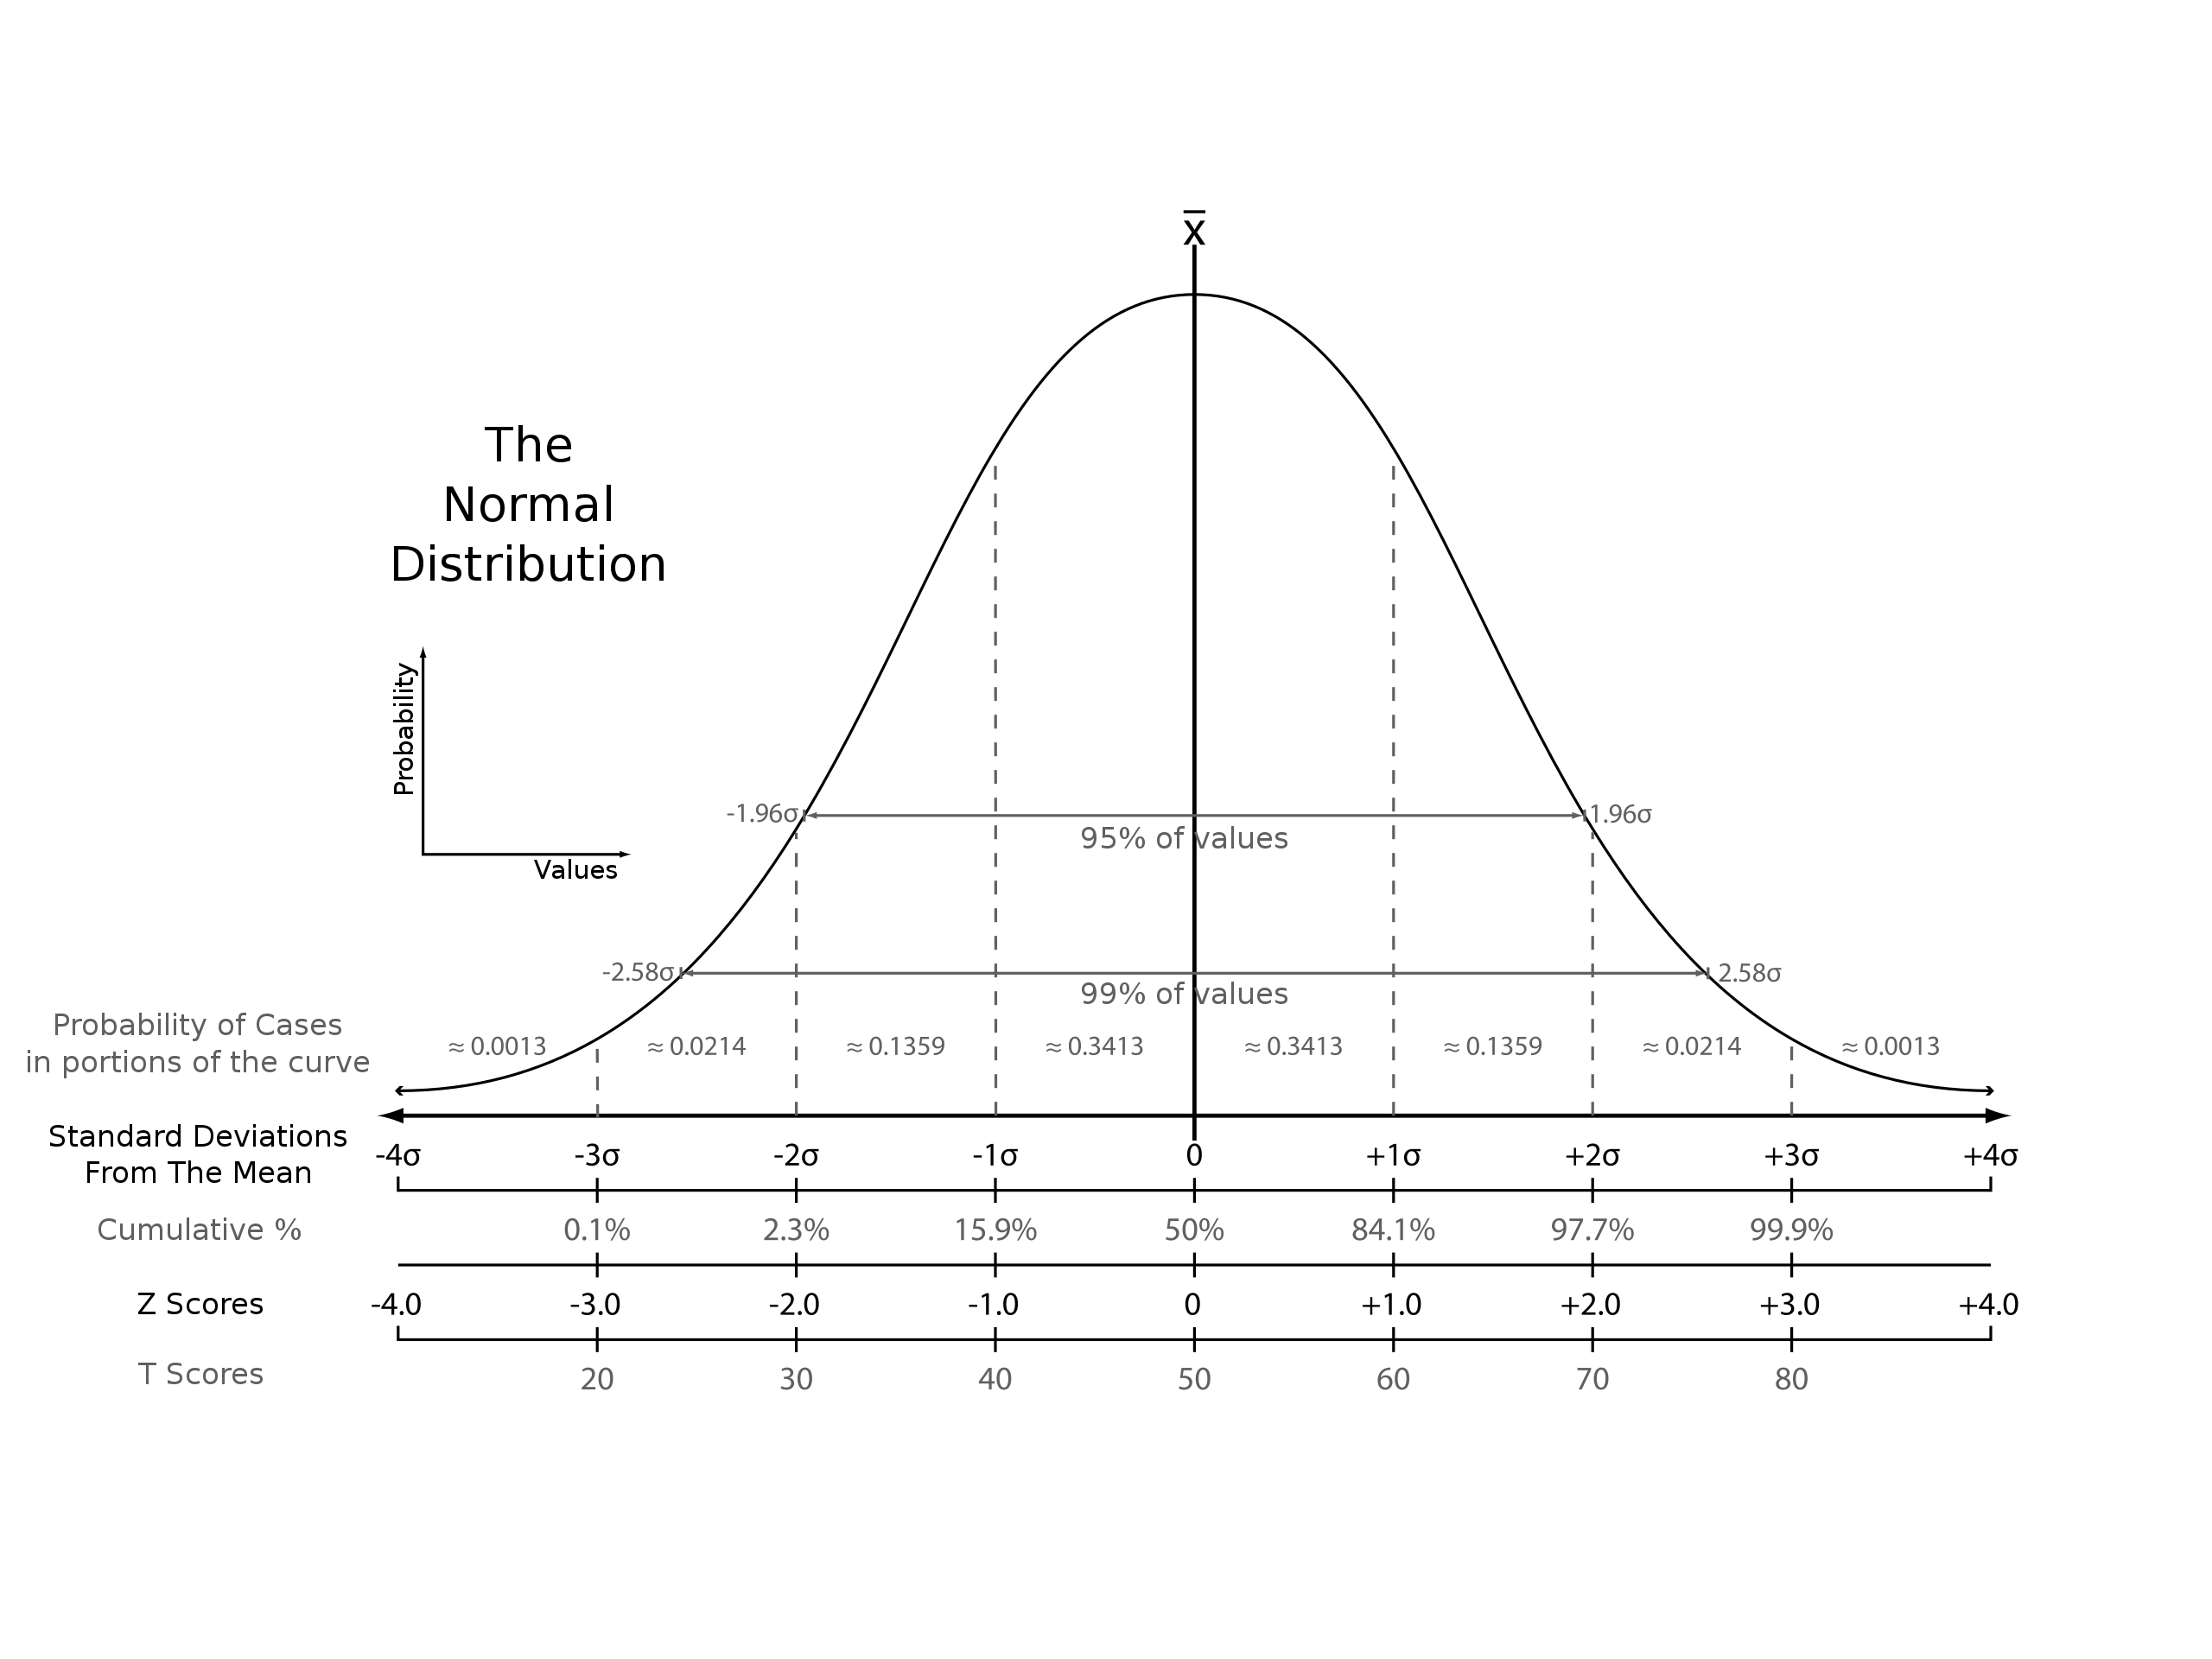
\includegraphics[scale=0.15]{The_Normal_Distribution.png}
	\caption[]{Compares the various grading methods in a normal distribution. Includes: Standard deviations, cumulative percentages, percentile equivalents, Z-scores, T-scores.}
	\label{zscorecompare}
	\end{center}
	\end{figure}

In educational assessment, T-score is a standard score Z shifted and scaled to have a mean of 50 and a standard deviation of 10.
